\documentclass[a4paper,12pt]{report}
\usepackage[utf8]{inputenc}
\usepackage{hyperref}
\usepackage[italian]{babel}
\usepackage[italian]{cleveref}
\usepackage{graphicx}


\title{\textbf{Traccia 2: Python Web Server}
Realizzazione di un server che gestisca un sito per un azienda ospedaliera}

\author{
\\Matteini Mattia
\\Paganelli Alberto
}
\date{\today}

\begin{document}

\maketitle

\tableofcontents


\chapter{Introduzione}

\section{Descrizione}
La piattaforma web realizzata elenca i principali servizi offerti dal Policlinico di Milano.
Riassume tutte le informazioni principali per usufruire di essi e le istruzioni necessarie per poter consultare esami, risultati o il proprio fascicolo sanitario.
\\
\\
Sarà presente una homepage del sito web contenente una piccola preview e descrizione  dei servizi offerti oltre ad un bottone per poter scaricare un pdf che raccoglie le informazioni più importanti relative alla struttura. 
\\
\\
Dalla homepage si possono visualizzare i servizi e si può navigare in pagine specifiche per ognuno di essi, all’interno di ogni pagina dedicata sarà presente anche un collegamento per tornare all’homepage.
\\
\\
Inoltre sarà possibile conoscere i volontari che si offrono all’aiuto dei cittadini nella sezione dedicata “Volontari”. 
All’interno di quest’ultima si potrà scaricare un elenco dei volontari nei quali sarà presente il numero di telefono ed un nominativo.
\\
\\
/* Il download dei pdf è stato fatto in maniera molto semplificata ed occorrerà sostituire il pdf in caso di aggiornamento. */
\\
\\
Un'ulteriore sezione è quella dei contatti nella quale l’utente potrà trovare un contatto mail oltre a link Linkedin e Facebook del Policlinico di Milano.


\clearpage

\section{Requisiti}

\begin{enumerate}
    \item \textsc{Il server dovrà mantenere più connessioni in contemporanea per garantire l'accesso a più utenti}
    \item \textsc{Nell’homepage dovranno essere presenti dei collegamenti ai servizi offerti}
    \item \textsc{Possibilità di scaricare un pdf per ogni servizio}
    \item \textsc{Interruzione dell'esecuzione opportunamente gestita}
    \item \textsc{Pagina HTML singola per ogni servizio}
\end{enumerate}
 


\chapter{Design}

\section{Client}

\clearpage

\section{Server}
Il server scritto in \textbf{Python} utilizza il package \texttt{socketserver} e in particolare la classe \textbf{ThreadingTCPServer} per gestire molteplici e semplici richieste alla volta.
Per la costruzione dell’istanza si inserisce nessun indirizzo locale nello specifico così in automatico riconoscerà l’accesso sia da localhost e da indirizzo ip del proprio computer nella rete al quale è connesso (esempio: 192.168.1.20.
Per la gestione delle richieste utilizziamo la classe \textbf{SimpleHTTPRequestHandler}, appartenente al package \texttt{http}, che è più che necessario per il nostro applicativo.
\\
\\
Come operazioni preliminari rendiamo utilizzabile lo stesso indirizzo IP a più richieste in entrata (\texttt{allow\_reuse\_address}), e poi facciamo si che quando il programma termina vengano terminati anche tutti i threads in sospeso generati dal server (\texttt{daemon\_threads}).
\\
\\
Successivamente definiamo un metodo che gestisca l’uscita dal programma e la chiusura del socket server, per questo utilizziamo il package \texttt{signal} che ci permette di intercettare i diversi segnali mandati al processo, in questo caso un SIGINT (2).
\\
\\
Infine abbiamo un \texttt{while True} dentro al quale chiamiamo il metodo \texttt{server\_forever} che dà vita a un nuovo thread che gestirà le richieste che arrivano e bloccherà il thread principale, inoltre lasciamo il \texttt{poll\_interval} di default che è di 0.5 secondi, quindi ogni mezzo secondo verrà controllato se viene ricevuto una richiesta di shutdown.


\section{Threading}

Per quanto riguarda la gestione di più richieste nello stesso momento, utilizzando un \textbf{ThreadingTCPServer} abbiamo un Main Thread avviato dal metodo \texttt{serve\_forever}, il quale crea un altro thread per ogni richiesta che arriva al server in modo da poterle gestire tutte contemporaneamente.


\chapter{Guida}
Per avviare il server basterà dare il seguente comando da terminale \texttt{"python server.py PORT"} dove PORT è il numero della porta che si vuole utilizzare per l’ascolto, se non si inserisce nessun parametro di default verrà utilizzata la porta 8080.


\begin{figure}[ht]
    \begin{center}
        \centering
        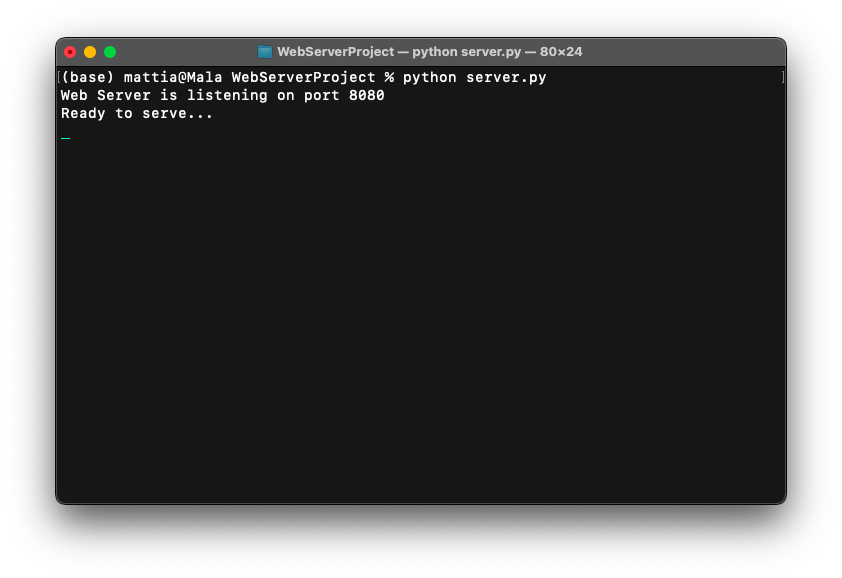
\includegraphics[width=\textwidth]{img/Terminale1.png}
    \end{center}
\end{figure}

\clearpage

Per visualizzare la pagina principale basterà avviare un browser e digitare il seguente link \texttt{"localhost:PORT/index.html"}, sostituendo PORT col numero di porta che si è data al server.
\\
\\
N.B. si può anche digitare l'indirizzo IP della macchina sulla quale sta girando il server al posto di utilizzare \texttt{"localhost"}.
\\
\\
\begin{figure}[ht]
    \begin{center}
        \centering
        
\includegraphics[scale=.8]{img/Link.png}
    \end{center}
\end{figure}
\\
\\
\begin{figure}[ht]
    \begin{center}
        \centering
        \hspace*{-0.8in}
        
\includegraphics[scale=.35]{img/Home.png}
    \end{center}
\end{figure}

\clearpage

Si può notare la gestione delle richieste effettuate dal browser verso il server, il quale risponde con i percorsi delle risorse necessitate dal browser per far visualizzare la pagina web (file, immagini, ecc...).
\\
\\
\begin{figure}[ht]
    \begin{center}
        \centering
        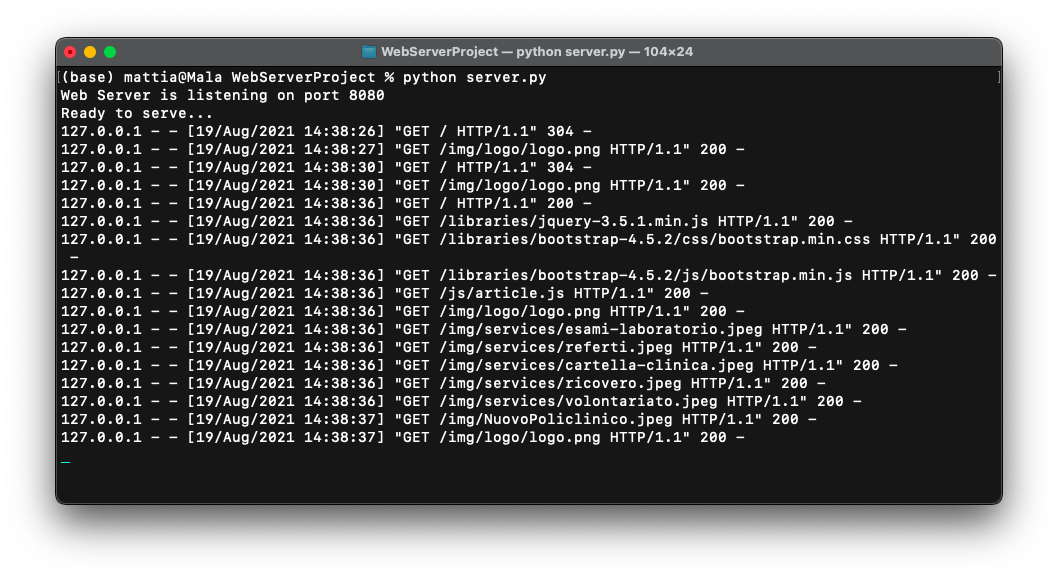
\includegraphics[width=\textwidth]{img/Terminale2.png}
    \end{center}
\end{figure}



\end{document}
